% ------------------------------------------------------------------------------
% TYPO3 CMS 7.2 - What's New (English Version)
%
% @author	Michael Schams <schams.net>
% @license	Creative Commons BY-NC-SA 3.0
% @link		http://typo3.org/download/release-notes/whats-new/
% @language	English
% ------------------------------------------------------------------------------
% LTXE-CHAPTER-UID:		93899f32-8efb477e-ed6973d2-b679bd8e
% LTXE-CHAPTER-NAME:	Backend User Interface
% ------------------------------------------------------------------------------

\section{Backend Gebruikersinterface}

% ------------------------------------------------------------------------------
% LTXE-SLIDE-START
% LTXE-SLIDE-UID:		7bb99d03-6678d1ca-e8710169-6b36a6ea
% LTXE-SLIDE-ORIGIN:	c151f95c-3fe3eb42-442ce244-5f987f80 English
% LTXE-SLIDE-TITLE:		Customized BE login form
% LTXE-SLIDE-REFERENCE:	unknown
% ------------------------------------------------------------------------------
\begin{frame}[fragile]
	\frametitle{Backend Gebruikersinterface}
	\framesubtitle{Aanpasbaar inlogscherm}

	Systeemextensie \texttt{backend} laat admin een eigen achtergrond, een logo
	en een kleur kiezen voor het backend inlogscherm:

	\begin{figure}
		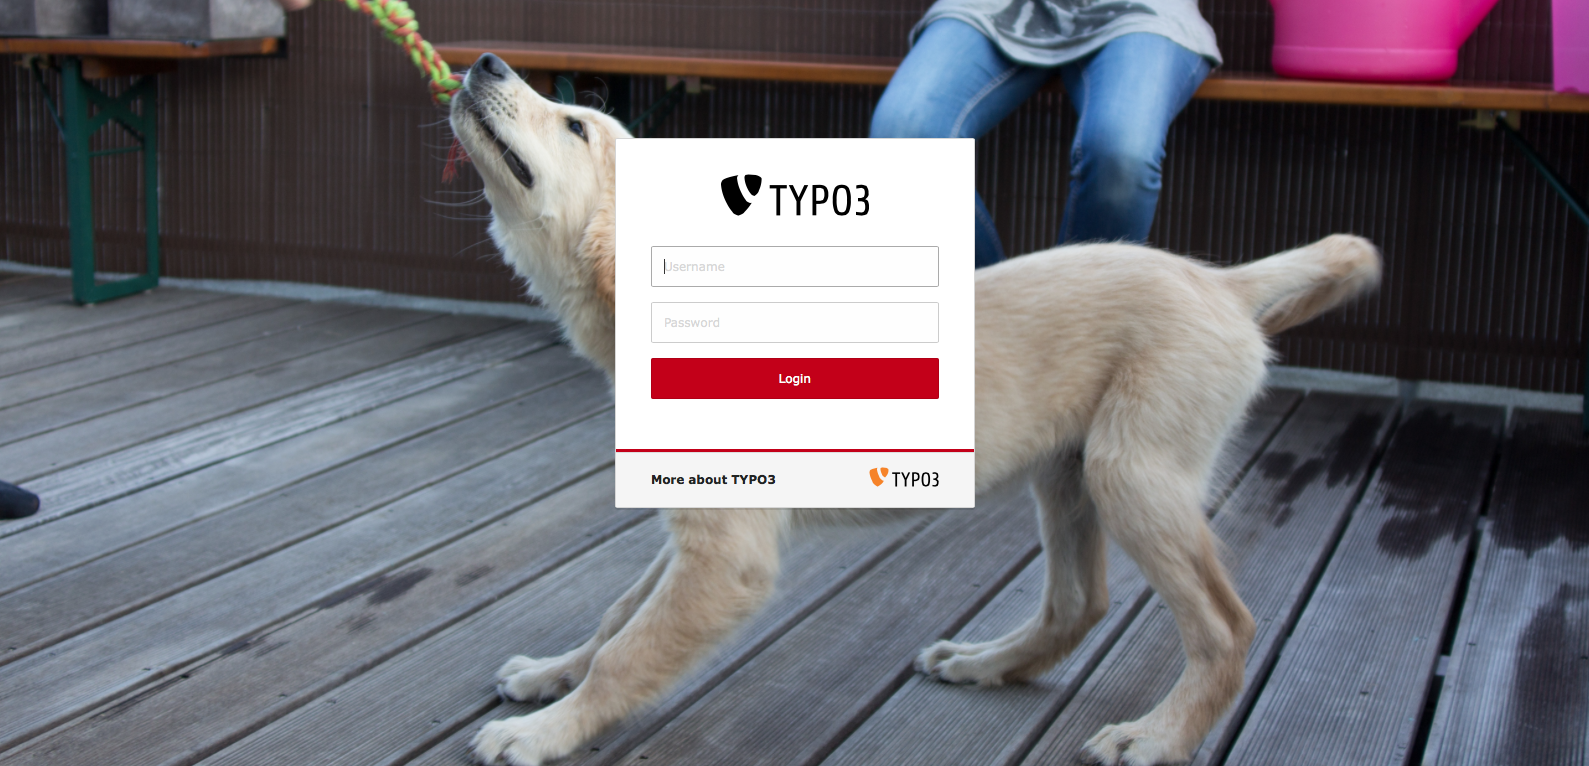
\includegraphics[width=0.75\linewidth]{BackendUserInterface/Login.png}
	\end{figure}

\end{frame}

% ------------------------------------------------------------------------------
% LTXE-SLIDE-START
% LTXE-SLIDE-UID:		d46b75b2-7da1ba4e-7ca5e2ef-7b52c0e7
% LTXE-SLIDE-ORIGIN:	e2e353ae-3b2b5c00-0cd7c57d-d97d22c9 English
% LTXE-SLIDE-TITLE:		Add image cropping
% LTXE-SLIDE-REFERENCE:	Feature-65584-AddImageCropping.rst
% ------------------------------------------------------------------------------
\begin{frame}[fragile]
	\frametitle{Backend Gebruikersinterface}
	\framesubtitle{Afbeeldingen wijzigen: afsnijden}

	Redacteuren kunnen afbeeldingen op maat snijden in de backend. Deze functie
	moet voor BE-gebruikers geactiveerd worden ("Exclude Fields"):

	\begin{figure}
		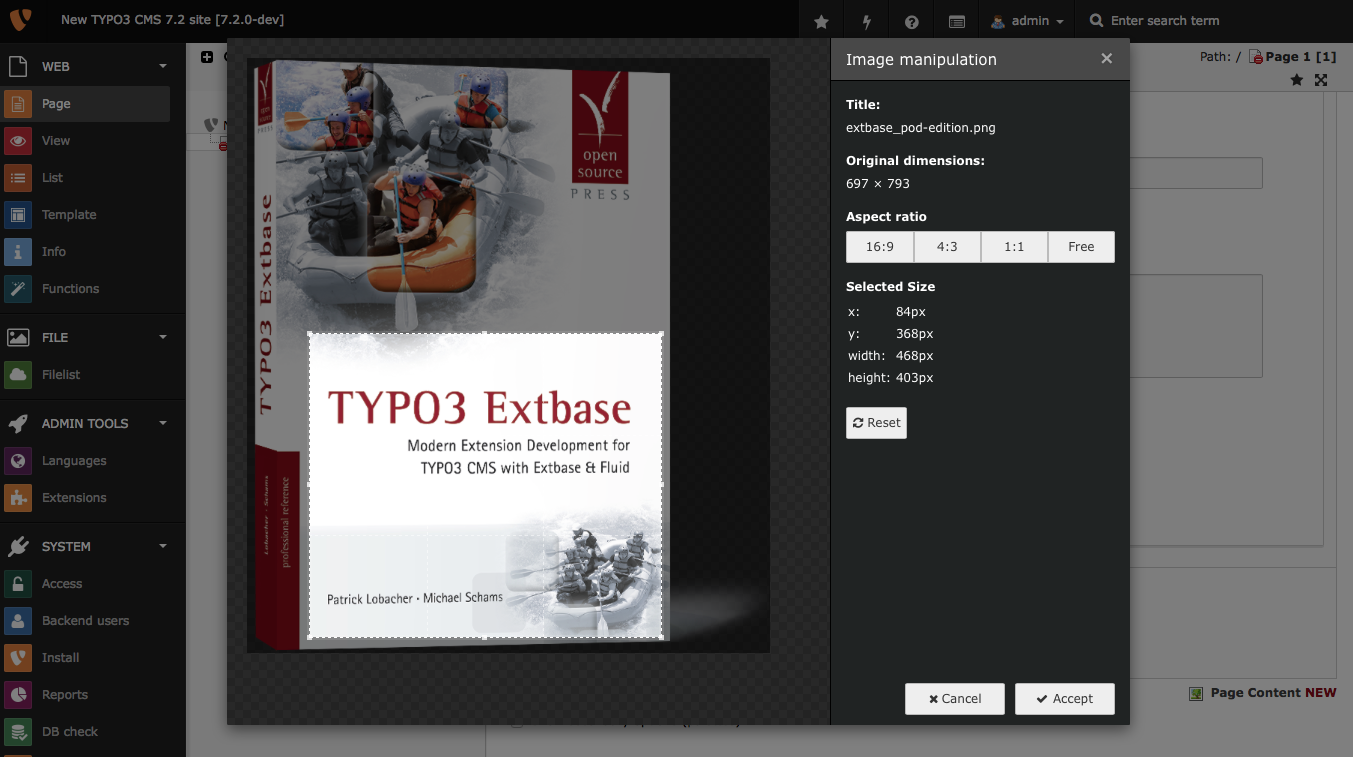
\includegraphics[width=0.7\linewidth]{BackendUserInterface/ImageCropping.png}
	\end{figure}

\end{frame}

% ------------------------------------------------------------------------------
% LTXE-SLIDE-START
% LTXE-SLIDE-UID:		9f75e5d0-a459c891-26f03240-bfc6be47
% LTXE-SLIDE-ORIGIN:	301dfea9-d2debf3e-dcaa7bcd-205e5990 English
% LTXE-SLIDE-TITLE:		Add backend user groups to backend user module
% LTXE-SLIDE-REFERENCE:	Feature-64686-AddBackendUserGroupsToBackendUserModule.rst
% ------------------------------------------------------------------------------
\begin{frame}[fragile]
	\frametitle{Backend Gebruikersinterface}
	\framesubtitle{Backend Gebruikersgroepen}

	Backend gebruikersgroepen kunnen in een submodule van de "Backend Gebruikers"
	module beheerd worden:

	\begin{figure}
		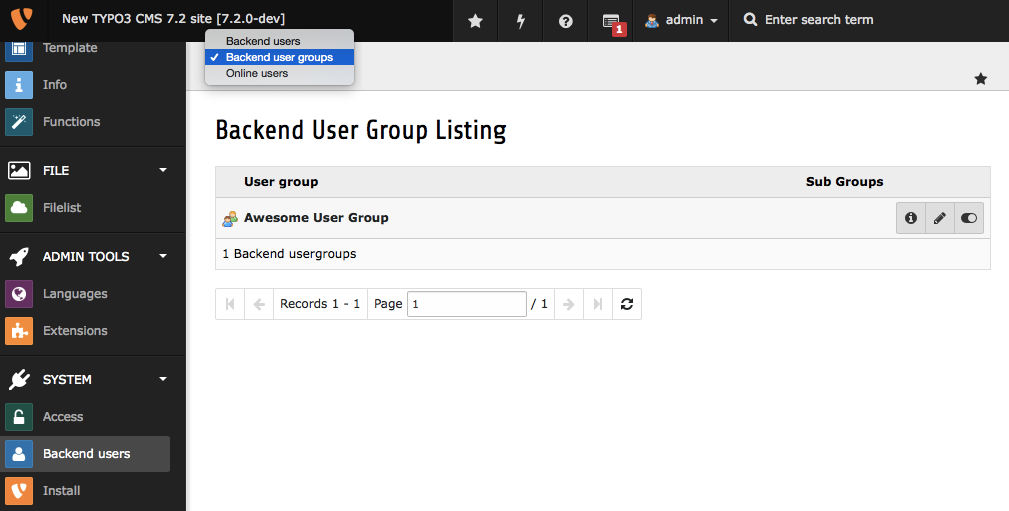
\includegraphics[width=0.70\linewidth]{BackendUserInterface/UserGroups.png}
	\end{figure}

\end{frame}

% ------------------------------------------------------------------------------
% LTXE-SLIDE-START
% LTXE-SLIDE-UID:		daa17f78-95d9f7de-421c689c-5630cad1
% LTXE-SLIDE-ORIGIN:	daa83c1e-08d2716b-de74cbda-42361551 English
% LTXE-SLIDE-TITLE:		Extension Manager: Disable automatic installation
% LTXE-SLIDE-REFERENCE:	Feature-50501-DisableAutomaticExtInstallation.rst
% ------------------------------------------------------------------------------
\begin{frame}[fragile]
	\frametitle{Backend Gebruikersinterface}
	\framesubtitle{Automatische installatie van extensies uitschakelen}

	Admins kunnen instellen dat Extensiebeheer gedownloade extensies
	niet meteen installeert:

	\begin{figure}
		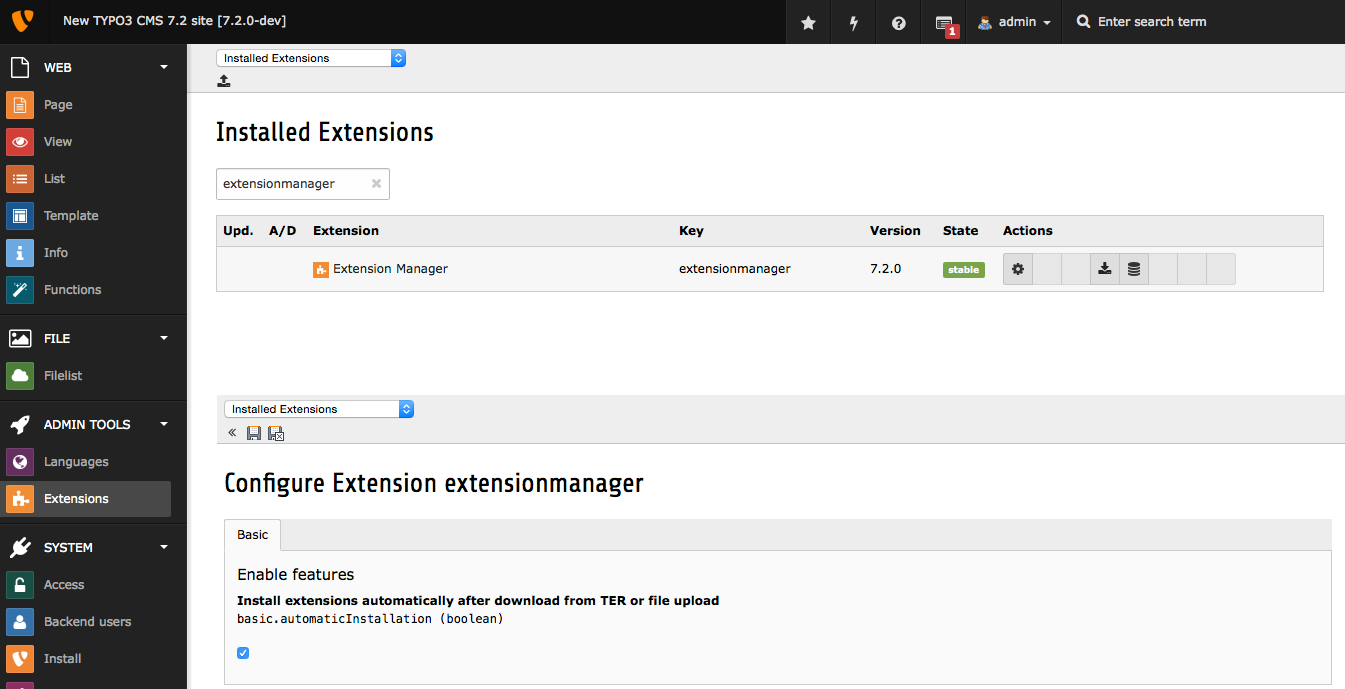
\includegraphics[width=0.70\linewidth]{BackendUserInterface/ExtManager.png}
	\end{figure}

\end{frame}

% ------------------------------------------------------------------------------
% LTXE-SLIDE-START
% LTXE-SLIDE-UID:		709cf2fa-c3ab2eac-da4671ba-12346d61
% LTXE-SLIDE-ORIGIN:	20769920-da9df227-c3b527b9-9a23bac1 English
% LTXE-SLIDE-TITLE:		Show remaining characters below text fields
% LTXE-SLIDE-REFERENCE:	Feature-66029-ShowRemainingCharactersBelowTextFields.rst
% ------------------------------------------------------------------------------
\begin{frame}[fragile]
	\frametitle{Backend Gebruikersinterface}
	\framesubtitle{Beschikbare tekens in tekstvelden}

	Het aantal nog beschikbare tekens wordt afgebeeld onder een tekstveld:

	\begin{figure}
		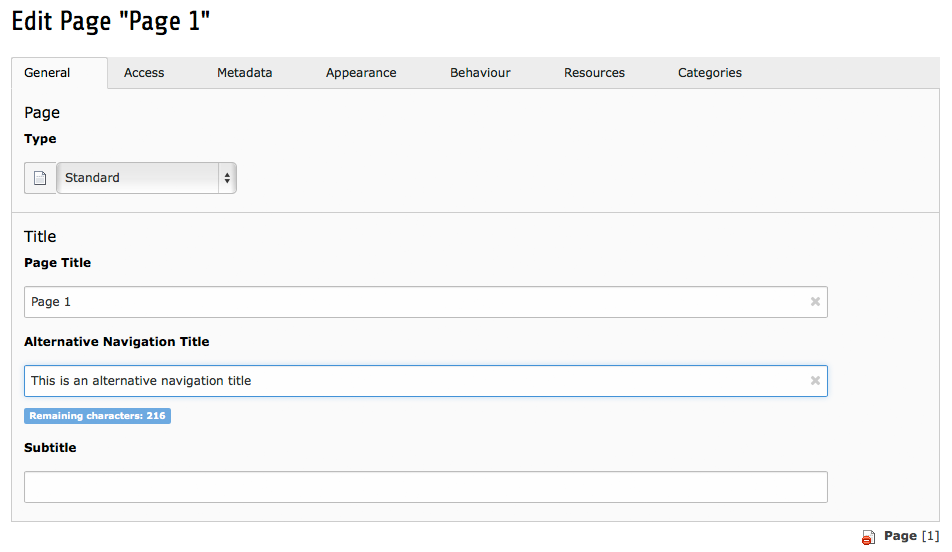
\includegraphics[width=0.70\linewidth]{BackendUserInterface/RemainingCharacters.png}
	\end{figure}

\end{frame}

% ------------------------------------------------------------------------------
% LTXE-SLIDE-START
% LTXE-SLIDE-UID:		50764742-0896e0c4-49215e45-fa6d4672
% LTXE-SLIDE-ORIGIN:	ff760b86-9d6b1ecd-d0e98565-f23c51f0 English
% LTXE-SLIDE-TITLE:		Show confirm message on closing an editform with unsaved changes
% LTXE-SLIDE-REFERENCE:	Feature-65996-AddConfirmationOnCloseEditformWithUnsavedChanges.rst
% ------------------------------------------------------------------------------
\begin{frame}[fragile]
	\frametitle{Backend Gebruikersinterface}
	\framesubtitle{Niet-bewaarde wijzigingen bevestigen}

	Een nieuw scherm waarschuwt redacteuren voor het verliezen van niet-
	opgeslagen wijzigingen:

	\begin{figure}
		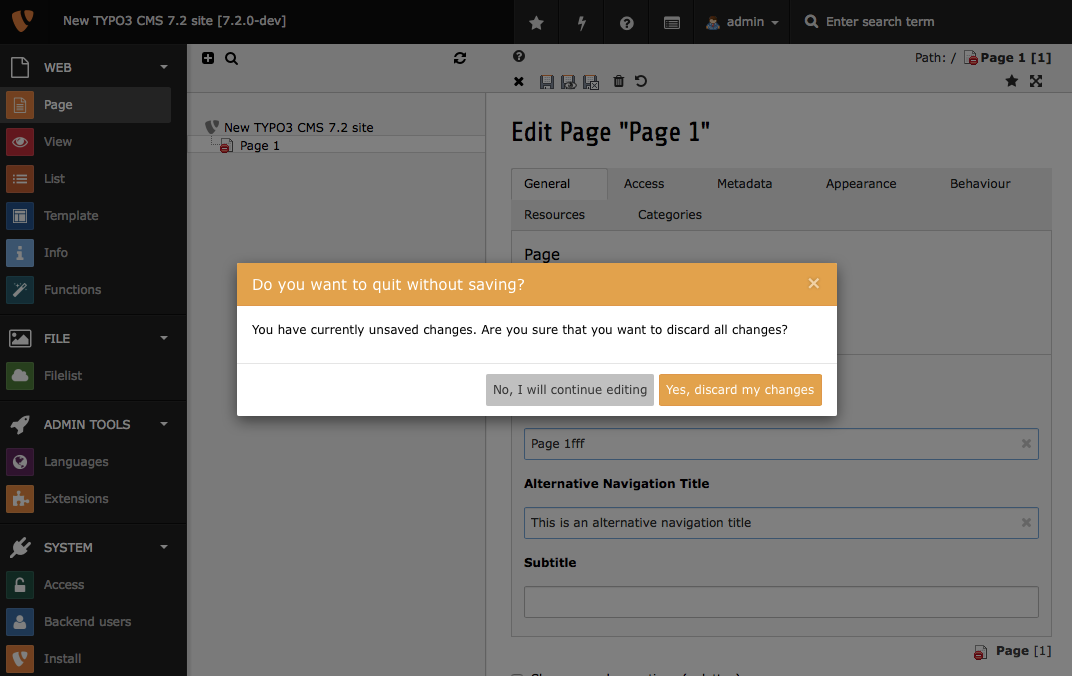
\includegraphics[width=0.65\linewidth]{BackendUserInterface/ClosingDialog.png}
	\end{figure}

\end{frame}

% ------------------------------------------------------------------------------
% LTXE-SLIDE-START
% LTXE-SLIDE-UID:		cc84cf0f-d25a541f-33d4d9d2-0bb93745
% LTXE-SLIDE-ORIGIN:	6ac9a35e-46541895-7509263e-28fb799f English
% LTXE-SLIDE-TITLE:		System Information Dropdown
% LTXE-SLIDE-REFERENCE:	Feature-65767-SystemInformationDropdown.rst
% ------------------------------------------------------------------------------
\begin{frame}[fragile]
	\frametitle{Backend Gebruikersinterface}
	\framesubtitle{Uitklapscherm systeeminformatie}

	Een uitklapscherm toont diverse gegevens over het systeem waar TYPO3 op
	geïnstalleerd is. Dit kan uitgebreid worden:\newline
	\small(zie hoofdstuk "Wijzigingen nader bekeken" voor meer details)\normalsize

	\begin{figure}
		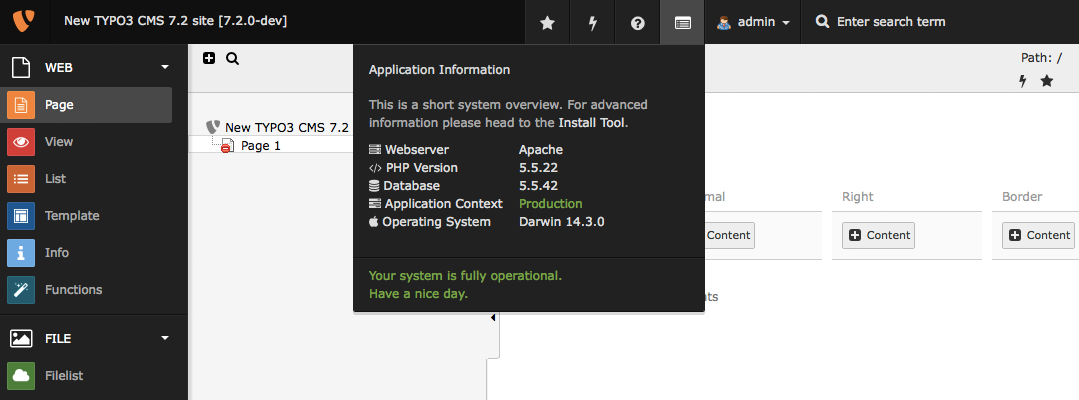
\includegraphics[width=0.85\linewidth]{BackendUserInterface/SystemInformation.png}
	\end{figure}

\end{frame}

% ------------------------------------------------------------------------------
% LTXE-SLIDE-START
% LTXE-SLIDE-UID:		d109a2a5-105ae94d-055fd30d-4c138bad
% LTXE-SLIDE-ORIGIN:	79a2ee0c-3439d600-08990adb-6bed8c19 English
% LTXE-SLIDE-TITLE:		Ask for old password when changing
% LTXE-SLIDE-REFERENCE:	commit bf6f5226eb6cb441bb53657a88ef42f1cdb5155f
% ------------------------------------------------------------------------------
\begin{frame}[fragile]
	\frametitle{Backend Gebruikersinterface}
	\framesubtitle{Wachtwoord wijzigen}

	Backend gebruikers moeten hun huidige (oude) wachtwoord invoeren om het te
	kunnen wijzigen in een nieuw wachtwoord:

	\begin{figure}
		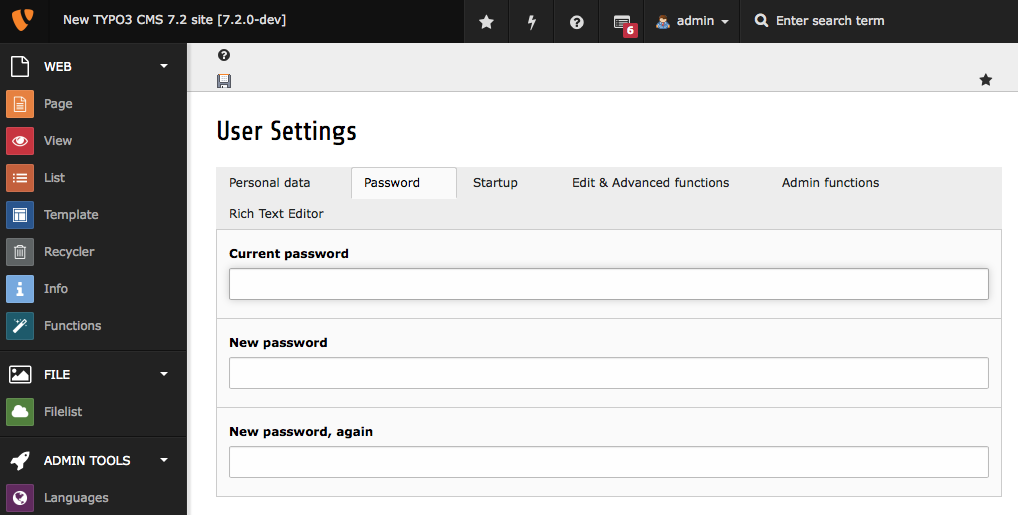
\includegraphics[width=0.7\linewidth]{BackendUserInterface/Password.png}
	\end{figure}

\end{frame}

% ------------------------------------------------------------------------------
% LTXE-SLIDE-START
% LTXE-SLIDE-UID:		6603f0e4-b3bf2a19-d15cfbfe-a57c3eda
% LTXE-SLIDE-ORIGIN:	7725bce9-e606f055-bf2e7b4a-e870fe2a English
% LTXE-SLIDE-TITLE:		Add icon for "Show Content From Page"
% LTXE-SLIDE-REFERENCE:	commit f8aa3eea9aed97a901ef0c3e7c650e1218839596
% ------------------------------------------------------------------------------
\begin{frame}[fragile]
	\frametitle{Backend Gebruikersinterface}
	\framesubtitle{Paginaicoon voor "Toon content van pagina"}

	Een nieuw icoon in de paginaboom laat zien dat een pagina inhoud van een andere
	pagina toont:

	\begin{figure}
		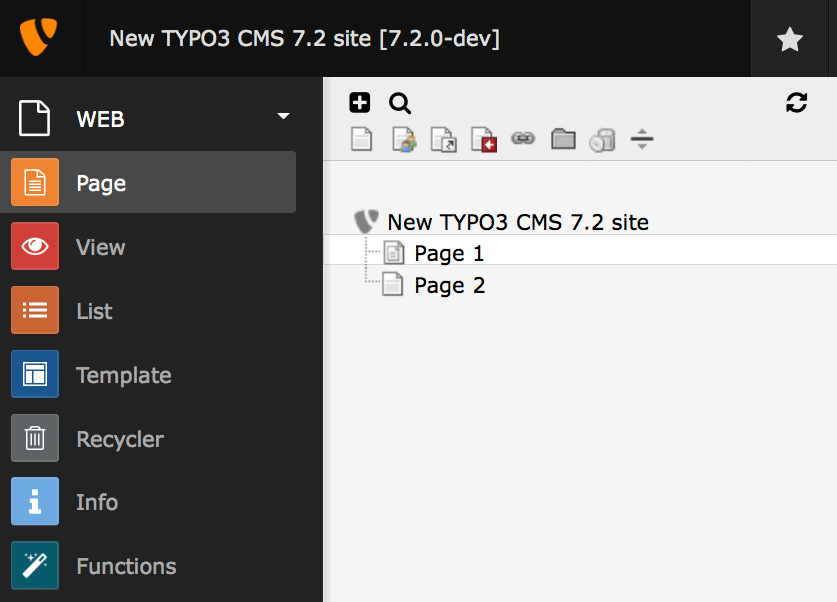
\includegraphics[width=0.45\linewidth]{BackendUserInterface/ShowContent.png}
	\end{figure}

\end{frame}

% ------------------------------------------------------------------------------
% LTXE-SLIDE-START
% LTXE-SLIDE-UID:		3bc47663-5c41749e-9fbce3c6-91b6f067
% LTXE-SLIDE-ORIGIN:	5ac2de45-9be12bf9-1c326192-602839fb English
% LTXE-SLIDE-TITLE:		Extension Manager: Choose version for update
% LTXE-SLIDE-REFERENCE:	commit a26396a4530b530744ec8b36c5fb5606789a6739
% ------------------------------------------------------------------------------
\begin{frame}[fragile]
	\frametitle{Backend Gebruikersinterface}
	\framesubtitle{Extensies bijwerken}

	Bij het bijwerken van een extensie kan nu gekozen worden welke versie
	geïnstalleerd moet worden:

	\begin{figure}
		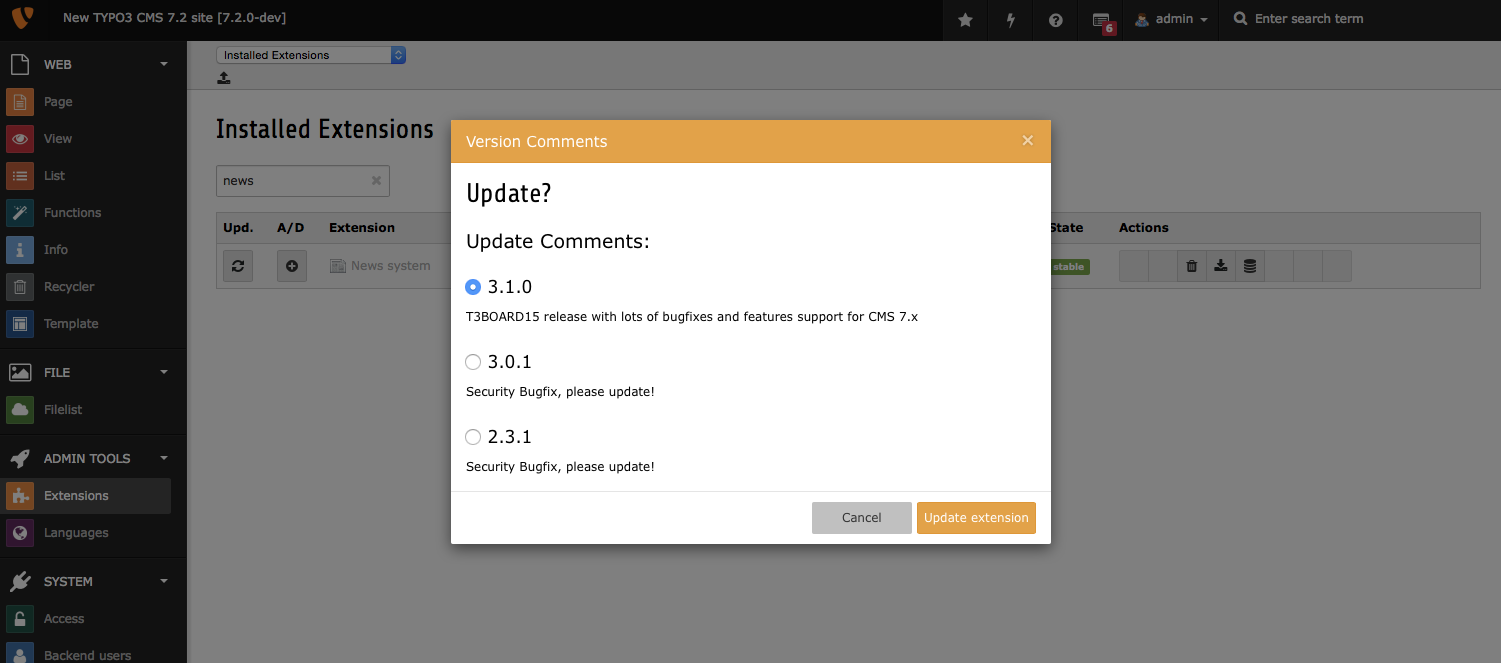
\includegraphics[width=0.75\linewidth]{BackendUserInterface/Update.png}
	\end{figure}

\end{frame}

% ------------------------------------------------------------------------------
% LTXE-SLIDE-START
% LTXE-SLIDE-UID:		205d82be-a099e4b5-d5dc09c1-0ff64a76
% LTXE-SLIDE-ORIGIN:	f6be31f7-155d676c-0e551545-3fc89e89 English
% LTXE-SLIDE-TITLE:		Add scheduler task to remove deleted records
% LTXE-SLIDE-REFERENCE:	Feature-32651-AddSchedulerTaskToRemoveDeletedRecords.rst
% ------------------------------------------------------------------------------
\begin{frame}[fragile]
	\frametitle{Backend Gebruikersinterface}
	\framesubtitle{Taak voor vuilnisbak}

	Een nieuwe taak voor de \texttt{recycler} gooit verwijderde records weg uit tabellen
	in de database. De maximale ouderdom en de schoon te maken tabellen kunnen
	ingesteld worden in de opties van de taak.
	\newline
	Dit kan ook gelden voor bestanden die in een contentelement gebruikt zijn.

	\begin{figure}
		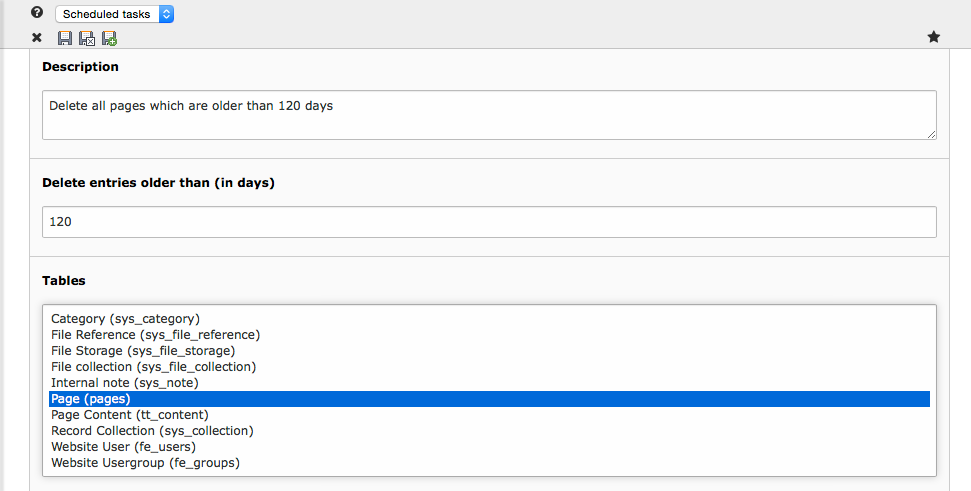
\includegraphics[width=0.68\linewidth]{BackendUserInterface/RecyclerTask.png}
	\end{figure}

\end{frame}

% ------------------------------------------------------------------------------
